
\section{Ejercicio 2: Menos es más}
    % 1. Describir detalladamente el problema a resolver dando ejemplos del mismo y sus soluciones.
	\subsection{Descripción del problema}

	\begin{figure}[ht]
		\begin{center}
			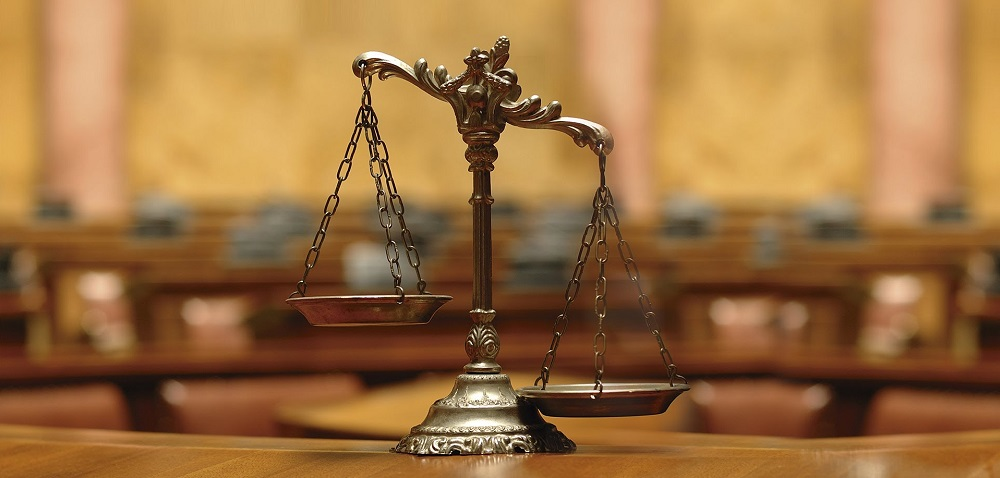
\includegraphics[width=0.5\columnwidth]{imagenes/balanza.jpg}
			\caption{Equilibro}
		\end{center}
	\end{figure}

	En su destino hacia la cruz en el mapa recorrieron varias salas distintas. Se dieron cuenta que en cada sala se iban encontrando con un fragmento de una tabla con un mansucrito antiguo. Por lo tanto, antes de continuar, quieren juntarlos todos.\par
	A medida que se iban abriendo camino se dieron cuenta que ciertas paredes derribables requerían cierto esfuerzo para
	abrirse. Este esfuerzo será representado por un $n\in{\mathbb{n}}$ donde $n < 10$. Luego, teniendo un mapa de $F*C$ (F = Filas y C = Columnas), donde se indique el $n$ en las paredes derribables, quieren encontrar cual es el mı́nimo esfuerzo que deben hacer para acceder a todas las salas. \par

	Por lo tanto, se deberá pasar por parametro al algoritmo, el mapa con sus paredes y el esfuerzo para romperlas. 
	\newline
	~

	\textbf{Formato de entrada:} La primer lı́nea consta de dos enteros positivos F y C, donde F es la cantidad de filas en el mapa, y C es la cantidad de columnas. Las siguientes F filas contienen C caracteres. Un “.” representa un lugar caminable, los números del 1 al 9 indican el esfuerzo en romper esa pared, un “\#” representa una pared indestructible. Las paredes con más de 2 paredes adyacentes son indestructibles (contendran un “\#”). Las paredes con menos de 2 paredes adyacentes son indestructibles (contendran un “\#”). Dos salas se pueden conectar si existe una pared adyacente a las dos salas que se puede destruir (Es decir, no quedan conectadas si se rompen muchas parede adyacentes). Por último, los bordes del mapa tendrán un “\#”.


	\begin{verbatim}
    F C
    F_1
    ...
    F_n
    \end{verbatim}
    

	~

	\textbf{Salida:} La salida consta de un número indicando el esfuerzo que debe hacer el equipo para acceder a todas las salas. Si no es posible recorrer todas las salas se imprime un −1. La salida tendrá el siguiente formato:\par
	
	\begin{tabular}{ll}
		\texttt{E}
	\end{tabular}



	~

	Se tiene como restricción que $F$ y $C$ está en el siguiente rango: 1$<=$ $F,C$ $<=$ $10^{4}$. La complejidad temporal debe ser a lo sumo $\ord(FC * \log{FC}{})$.

    % 2. Explicar de forma clara, sencilla, estructurada y concisa, las ideas desarrolladas para la resolución del problema. Utilizar pseudocódigo y lenguaje coloquial (no código fuente). Justificar por qué el procedimiento resuelve efectivamente el problema.
    
    \subsection{Solución propuesta}

    \subsubsection{Modelo}

    Para resolver este problema, se pedía encontrar el mínimo esfuerzo, para pasar por todas las salas del mapa. Para esto se usó el algoritmo de Kruskal, cuyo fín es encontrar el \textbf{Arbol Generador Mínimo} dentro de un grafo, cuyo pesos en las aristas sea positivo. En nuestro caso, esto representaría el mínimo esfuerzo, para poder visitar todas las salas. Para poder usar Kruskal, modelamos el problema en grafos. Para esto, se creó una matriz de $F*C$, donde fueron guardados los caractéres del mapa pasados como parámetro de entrada.\par
    Luego se usó esta matríz para generara los nodos y las aristas. Para esto, en principio cada posicion de la matriz es un nodo, numerados según la posición dentro de la matriz ($filaDelNodoActual * cantColumnas + columnaDelNodoActual$). \par
    Una vez generada la matríz, se la vuelve a recorrer, para generar las aristas. Sea nodoActual, el caracter ubicado en la posición de la matríz en la cual estoy queriendo generar una arista,

    \begin{itemize}
    	\item Si nodoActual es '\#', no hago nada.
    	\item Caso contrario, me fijo si nodoActual es '.' o un número.
    	\begin{itemize}
    			\item Si es un '.'. Se debe fijar en la columna siguiente de la matriz, este nodo lo llamaremos, nodoVecino.\par
 		   		Si nodoVecino es distinto de '\#'. Genero una arista, cuyo comienzo es el número de nodoActual, su fin es el de nodoVecino, y el peso es 0. Análogo para la posición inmediata dentro de la matriz, de la fila siguiente.
  		  		\item Si es un número. Deberá hacer lo mismo que en el caso anterior. Con la diferencia que, si uno de sus vecinos es también un número, no deberá hacer nada y que solo tendrá un vecino '.', en la columna inmediata superior o, en la fila siguiente, dentro de la matriz, y cuyo peso de la arista, será el número del nodo.
 			   	\end{itemize}
    \end{itemize} 


    Luego para el siguiente mapa,

       	\begin{figure}[h]
		\begin{center}
			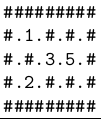
\includegraphics{imagenes/altoMapa.png}
			\caption{Mapa a modelar}
		\end{center}
	\end{figure}


    Queda el siguiente grafo,
    
   	\begin{figure}[h]
		\begin{center}
			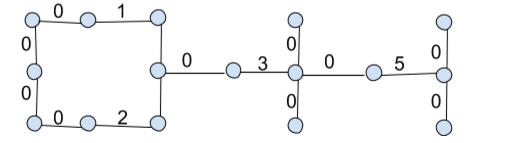
\includegraphics{imagenes/grafoOK.png}
			\caption{Grafo del mapa}
		\end{center}
	\end{figure}



    Cada una de estas aristas, es guardada en un vector de aristas.
    Luego, este vector de aristas, es usados en el algoritmo de Kruskal, quien devolverá la suma del \textbf{Arbol Generador Mínimo}. En caso de no tener solución, es decir, no poder recorrer el mapa, devolverá -1.





	\subsubsection{Implementación}\label{ej2_imp}

	Habiendo introducido la idea, se detalla el comportamiento del algoritmo para
	una entrada con $P$.

	Se presenta un pseudocódigo para tener de referencia al seguir la
	explicación detallada a continuación:

	\begin{codesnippet}
	\begin{verbatim}
	izquierda = verdadero
	divisiones = 0
	izquierdas = []
	derechas = []
	Mientras p != 0
	    cociente = p / 3
	    resto = p - (cociente *3)
	    Si resto es 0
	      Si no lo puse en izquierda al anterior
	        Agrego a izquierdas la pesa con valor (3 ^ divisiones)
	      izquierda = verdadero
	    Si resto es 1
	      Si anterior lo puse en izquierda
	        Agrego a izquierdas la pesa con valor (3 ^ divisiones)
	      Si no
	        Agrego a derechas la pesa con valor (3 ^ divisiones)
	    Si resto es 2
	      Si anterio lo puse en izquierda
	        Agrego a derechas la pesa con valor (3 ^ divisiones)
	      izquierda = falso
	    p = cociente
	    divisiones += 1
	Fin Mientras
	Si el último no lo puse en la izquierda
	   Agrego a izquierdas la pesa con valor (3 ^ divisiones)
	\end{verbatim}
	\end{codesnippet}

	\begin{enumerate}
		\item{
			La primera parte consiste en la inicialización de valores para el algoritmo. Se tiene una variable booleana que indica en qué platillo fue colocada la última pesa para cada iteración. Esta variable se inicializa en verdadera y es utilizada para saber en qué platillos hay que colocar las pesas que siguen. Esta variable es muy importante ya que determina en qué casos se van a reemplazar dos pesas de una potencia de 3, por otras pesas y cómo hacerlo. La variable divisiones es simplemente un índice que representa la cantidad de divisiones realizadas al número P. Por último se tienen dos listas inicializadas vacías, que van a almacenar las pesas que hay que colocar en los platillos izquierdo y derecho.
		}

		\item{
			El ciclo principal se ejecuta mientras P sea distinto de cero. En el cuerpo del ciclo se realiza la división del número P por 3 y se almacenan en dos variables distintas el cociente y el resto de dicha operación. Para el caso del valor del resto se tienen 3 posibilidades:
			\begin{enumerate}
				\item{
					EL resto es igual a 0: En este caso hay que preguntar si la anterior pesa fue colocada o no en el platillo derecho. Si fue colacada en el platillo derecho, se agrega a la lista de izquierdas la pesa que corresponde al valor (3$^{divisiones}$). La variable izquierda se actualiza con el valor verdadero, indicando que la última pesa fue colacada del lado izquierdo.
				}
				\item{
					El resto es igual a 1. En este caso tenemos dos posibilidades distintas:
					\begin{enumerate}
						\item{
							La anterior pesa fue colocada del lado izquierdo, por lo tanto esta pesa también tiene que colocarse del mismo lado. Se agrega entonces a la lista de izquierdas el valor (3$^{divisiones}$).
						}
						\item{
							La anterior pesa fue colocada del lado derecho, por lo tanto esta pesa también tiene que colocarse del mismo lado. Se agrega entonces a la lista de derechas el valor (3$^{divisiones}$).
						}
					\end{enumerate}
				\item{
					El resto es igual a 2: Sólo basta con fijarse si la anterior pesa fue colacada en el platillo izquierdo. De ser así, se debe agregar a derechas la pesa con el valor (3$^{divisiones}$).
				}
				}
				\end{enumerate}
			}
			\item{
			    Lo último que se realiza en el ciclo es actualizar el valor de P, el cual va a contener el valor del cociente calculado al principio. De esta manera el valor de P se irá decrementando en cada ciclo hasta llegar a cero. También se suma uno al índice de divisiones.
				Finalmente, se pregunta si la última pesa fue colocada en la lista de derechas. De ser así, se agrega a la lista de izquierdas la pesa con valor (3$^{divisiones}$).
			}
	\end{enumerate}

	\subsubsection{Demostración de correctitud}

	Habiendo visto cómo funciona el algoritmo desarrollado, se procede a
	justificar por qué devuelve una solución. Para esto se explicará el algoritmo en base a las justificaciones matemáticas realizadas en la solución propuesta.
	\subsubsection*{Correctitud de ciclo}

	Lo que se va a demostrar a continuación es que el ciclo principal termina y calcula la solución al problema.

	El ciclo se ejecuta mientras P sea distinto de cero. Es decir termina cuando P es 0 y esto ocurre ya que lo que se hace en el ciclo es dividir el número P por 3 y reemplazar P por el resultado (cociente) de esta división en cada iteración. Eventualmente el cociente va a ser cero, por los teoremas de división entera y de desarrollo en base $d$. Lo que se está haciendo es utilizar el algoritmo de división para obtener el desarrollo en base 3 del número $P$. Los restos en cada iteración son los que indican que símbolos hay que utilizar para la representación del número en esa base. En este caso no interesa obtener la representación del número en base 3, sino trabajar con los símbolos en su desarrollo (restos). El resto de la división sólo puede ser 0, 1 o 2 (por el teorema de la división entera).

	A continuación se analiza la parte fundamental del algoritmo que consiste en la identificación de qué pesas utilizar y en qué platillos colocarlas dependiendo del resto. Se tienen las siguientes posibilidades: 

	\begin{enumerate}
		\item{
			Resto == 0. En este caso, si la última pesa fue colocada del lado izquierdo no hay que realizar nada. Esto es porque el anterior dígito en el desarrollo era o bien otro cero o un 1. Por lo tanto no es necesario utilizar esta pesa para compensar una de un valor menor que no pudo ser utilizada porque se estaban usando dos (esto fue explicado en la solución propuesta). En cambio si la anterior pesa fue colocada del lado derecho es porque el anterior dígito en el desarrollo del número era un 2. En este caso, hay que utilizar esta pesa, por lo que se agrega a la lista de izquierdas el valor de la potencia de 3 correspondiente. Independientemente de si se utilizó esta pesa o no, la variable izquierda se actualiza con el valor verdadero, ya que el hecho de que no se use una pesa de una determinada potencia también se toma como que se 'usó'' la pesa de la izquierda. Esto es porque en el caso de que el siguiente dígito en el desarrollo sea un uno, se tiene que poder distinguir si el anterior fue un 0 o un 2, lo cual no se podría realizar si no se actualiza el valor de esta variable. En la explicación del caso del resto 1 se puede entender mejor esta conclusión. 
		}
		\item{
			Resto == 1. En este caso siempre hay que agregar una pesa. Si el valor de la variable izquierda es verdadero (esto es porque el anterior dígito fue un 0 o un 1) hay que agregar esta potencia de 3 a la lista de izquierda. En el caso contrario significa que el anterior dígito era un 2 y como se demostró en la solución propuesta hay que colocar esta pesa en el lado derecho, ya que si el anterior fue un 2 hay que tomar este dígito, lo que lo convertiría de un 1 a un 2, y por lo tanto hay que aplicar nuevamente la fórmula propuesta. Por lo tanto en este último caso se agrega la potencia de 3 correspodiente en la pesa derecha. El valor de la variable izquierda no es necesario actualizarlo ya que si se agrega a la lista de izquierdas hay que modificarlo por verdadero (lo cual ya ocurre porque se agrega solamente a izquierdas si es verdadero) y si se agrega a la lista de derechas hay que modificarlo por falso (lo cual ya ocurre porque se agrega solamente a derechas si es falso).
		}
		\item{
			Resto == 2. En este caso se usa también la idea planteada en la solución al problema. Se agrega a la lista de derechas la pesa con el valor de la potencia de 3 correspondiente solamente si la anterior fue colocada en el lado izquierdo (es decir el anterior dígito es un cero o un uno) ya que si el anterior era un 2 no hay que realizar nada (por lo visto en la demostración de la solución). Finalmente se actualiza el valor de izquierda y se pone en falso siempre, ya que es necesario para el siguiente dígito en el desarrollo, ya que como se vió si el siguiente es cero va a haber que tomar la siguiente pesa y si es un 1 va a haber que colocar la pesa en el lado derecho.	
		}
	\end{enumerate}

	Como el ciclo finaliza cuando P es igual a cero, se puede dar el caso de que el último dígito en el desarrollo del número en base 3 (el más significativo) sea un 2. Por lo tanto y sabiendo que no sigue ningún dígito más, lo que hay que hacer si se da este caso es tomar esta pesa por lo visto en la solución.

	En conclusión lo que hace el algoritmo es dividir iterativamente el número por 3, obteniendo de esta forma su desarrollo en base 3 y al mismo tiempo colocando las pesas correspondientes en base a los restos obtenidos (teorema de desarrollo en base $d$). No es necesario obtener primero la representación del número en la base y después aplicar la solución; se puede realizar mientras se obtiene, tomando decisiones en base al resto de la división en cada iteración. La idea propuesta garantiza que el algoritmo siempre va retornar una solución por lo visto en la sección de "Solución". Las decisiones que se toman con los restos son las inferidas por la solución propuesta: si el dígito es 0, no se toma esa pesa salvo que el anterior sea un 2. si el dígito es 1, si el anterior es 0 o 1 se toma esa pesa, sino se resta la pesa; finalmente si el dígito es 2, si anterior es 2 no se toma ninguna acción y si no se resta la pesa. Además el algoritmo de división garantiza que las pesas que se toman, van a estar ordenadas de menor a mayor cumpliendo con la restricción del problema.

    % 3. Deducir una cota de complejidad temporal del algoritmo propuesto y justificar por qué el algoritmo cumple la cota dada. Utilizar el modelo uniforme.
	\subsection{Complejidad teórica}

	Para calcular la complejidad teórica de la solución propuesta se hará
	referencia a la sección \ref{ej2_imp} donde se posée el pseudocódigo junto a
	su explicación.

	El algoritmo tiene una complejidad temporal de $\ord(log(n))$, por lo tanto es
	logarítmico y cumple con la restricción de complejidad del enunciado. Esto se justifica con el hecho de que el algoritmo posee un ciclo
	principal que se ejecuta mientras $P$ sea distinto de cero, es decir desde el número $P$ hasta el número 0. En cada iteracion el tamaño de $P$ se reduce a un tercio, ya que se divide por 3. Por lo tanto el ciclo se ejecuta la cantidad de símbolos necesarios para obtener el número $P$ en base 3. Si $P$ requiere de $n$ símbolos es que:

	\newline
	$d^{n-1} <= P < d^n$

	\newline
	es decir, $n -1 <= log_3(P) < n$, lo que implica que $[log_3(P)] = n - 1$ y por lo tanto $n = [log_3(P)] + 1$


	Dentro del ciclo sólo se hacen comparaciones que tienen un costo asociado de $\ord(1)$, una división, una multiplicación y una resta de enteros (costo $\ord(1)$), una asignación y una suma, y se agregan elementos a una lista (todas estas operaciones tambien en $\ord(1)$). Por lo tanto se concluye que la complejidad del ciclo es $\ord(log(n))$. Fuera del ciclo sólo se realizan incializaciones de variables $\ord(1)$ al principio del algoritmo y una comparación e inserción en una lista al final también en $\ord(1)$. Por álgebra de órdenes de funciones, la complejidad temporal resultante del algoritmo es $\ord(log(n))$. 

    % 4. Dar un código fuente claro que implemente la solución propuesta. Se deben incluir las partes relevantes del código como apéndice del informe impreso entregado.

    \subsection{Experimentacion}
         

	Se realizaron pruebas experimentales para verificar que el tiempo de
	ejecución del algoritmo cumpliera con la cota asintótica de $\ord(log(n))$,
	demostrada teóricamente. Para ello fue necesario modificar el algoritmo propuesto, ya que como la complejidad está definida por la cantidad de símbolos necesarios para la representación del número en base 3 y se explicó que la misma era $log_3$ del número más uno, no se observan grandes diferencias en el tiempo de ejecución para números 'razonables', es decir números que puedan ser representados de una forma práctica y eficiente en C++. Por ejemplo para el caso de un número muy grande como $3^{30}$, la cantidad de iteraciones que va a realizar el ciclo es sólo 31, que no es muy diferente a la cantidad de iteraciones necesarias para el número $3^{3}$ (4 iteraciones) que es mucho menor. Los tiempos de ejecución de estas instancias son muy similares y dado a que hay muchas variables en cuestión cuando se corren (otros procesos que interfieren, atención de interrupciones y scheduling del S.O, etc) puede hasta darse el caso de que tarde más una instancia menor que una mayor. Se presenta la siguiente modificación del algoritmo para realizar las pruebas:

	\begin{codesnippet}
	\begin{verbatim}
	izquierda = verdadero
	divisiones = 0
	izquierdas = []
	derechas = []
	Mientras v.size != 0
	    Si v[size -1] = 0
	      Si no lo puse en izquierda al anterior
	        Agrego a izquierdas la pesa con valor (3 ^ divisiones)
	      izquierda = verdadero
	    Si v[size -1] = 1
	      Si anterior lo puse en izquierda
	        Agrego a izquierdas la pesa con valor (3 ^ divisiones)
	      Si no
	        Agrego a derechas la pesa con valor (3 ^ divisiones)
	    Si v[size -1] = 2
	      Si anterio lo puse en izquierda
	        Agrego a derechas la pesa con valor (3 ^ divisiones)
	      izquierda = falso
	    v.size -= 1
	    divisiones += 1
	Fin Mientras
	Si el último no lo puse en la izquierda
	   Agrego a izquierdas la pesa con valor (3 ^ divisiones)
	\end{verbatim}
	\end{codesnippet}

	Este algoritmo a diferencia del original, recibe como parámetros un arreglo de enteros (v) que representa el desarrollo en base 3 de un número y un entero que es el tamaño del arreglo. El arreglo de enteros puede contener por lo tanto en cada posición un entero entre 0 y 2 inclusive. El arreglo se interpreta como que en la posición 0 está el dígito más significativo y en la última el menos significativo.
	Con esta idea se puede realizar un mejor análisis del rendimiento del algoritmo ya que se pueden simular números mucho más grandes. Se puede tomar un arreglo de 5000 posiciones, lo cual representaría un número muy grande en base 3 que no se puede representar directamente. La idea es que este algoritmo realiza en el fondo lo mismo que el anterior, ya que lo que se hace es recorrer el arreglo (ciclo principal) y después tomar las mismas decisiones que en el original en base a los valores contenidos en cada posición del arreglo. Es decir lo que determina la complejidad en este caso es el tamaño del arreglo, pero el mismo por lo expuesto anteriormente es igual al logaritmo en base 3 de un número P cualquiera, el cual sería el resultante de realizar la descomposición del desarrollo.

	Para las pruebas lo que se realizó es probar con arreglos de tamaño 1 hasta 4600. Para estandarizar y que no haya constantes diferentes para cada arreglo (ya que lo que se hace depende del valor de cada posición) en todos los casos se completaron todas las posiciones de los arreglos con el valor 1, para que el tiempo esté determinado sólo por el tamaño del arreglo. Además cada uno de los arreglos es testeado 5000 veces para disminuir los outliers. Lo esperable es que haya una relación lineal entre el tiempo de corrida y el tamaño del arreglo, pero el mismo se debe interpretar como que la relación es logarítmica entre el número que representa el arreglo y el tiempo.Se utilizó para que esto se visualice mejor la escala logarítica, como se puede observar en el siguiente gráfico:  


    \renewcommand\constante{5}

	\begin{figure}[H]
      \begin{center}
        \includegraphics[width=0.7\columnwidth]{imagenes/ejercicio2.jpg}
        \caption{}
      \end{center}
  \end{figure}

El análisis expuesto de los datos recopilados presenta evidencia empírica sobre la cota de complejidad
demostrada teóricamente. Además se logra ver que la complejidad depende estrictamente de la cantidad
de símbolos que hay que utilizar para el desarrollo del número en base 3.